\chapter{Stand der Technik \& technische Grundlagen}
%Einleitung



\section{Drucktechniken}
%TODO Bilder
\label{drucktechniken}
	Dreidimensionale Objekte k�nnen mit verschiedenen Verfahren gedruckt werden. Viele werden bereits seit Langem eingesetzt. Die Technologie war folglich schon verf�gbar. In den letzten Jahre erreichen die Drucker den Endkundenmarkt. Grund daf�r sind eine Vielzahl von g�nstigen Druckern, die au dem Markt erh�ltlich sind. Im Folgenden sind verschiedene Druckverfahren erl�utert.
	
	\subsection{Schmelzschichtverfahren}%TODO
		Das verfl�ssigte Material wird durch eine D�se, den Extruder, auf eine Druckfl�che gepresst. Dort h�rtet es aus. Durch Bewegen des Druckkopfes �ber die Druckfl�che l�sst sich Schicht f�r Schicht ein Objekt auftragen.
		
		\piccaption{Prinzip des Schmelzschichtverfahrens \cite{gebhardt2004grundlagen}\label{fig:sdt:schmelzschicht}}
		\parpic{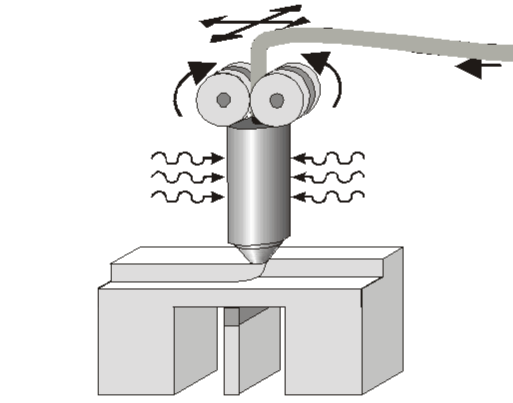
\includegraphics[width=.5\textwidth]{images/SdT/verfahren/extrusion_gebGr}}
 		\picskip{0}
 		\vspace*{3em}
		
		
		Das im Verh�ltnis zu anderen Drucktechniken langsame Verfahren eignet sich f�r die Erstellung von Modellen f�r das Testen von Passgenauigkeit.
		Die Auswahl an Materialien ist gro�; auch Lebensmitteldrucker wie solche f�r Schokolade sind m�glich. Im Gegensatz zu den meisten anderen Verfahren eignen sich Drucker dieses Verfahrens f�r den B�rogebrauch. Zudem sind mittlerweile preiswerte Drucker dieses Verfahrens erh�ltlich.
		
		\cite[S.17]{hagl2014_3DKompendium}
	 
	
	\subsection{Stereolithographie}
		\label{drucktechniken:stereolithographie}
		Das dreidimensionale �quivalent zum Rasterdruck baut Objekte aus Schichten von Rasterpunkten auf.
		
		Manche organischen Verbindungen k�nnen mittels \ac{UV}- Licht polymerisiert werden. Dadurch wird aus einem fl�ssigen Grundstoff ein fester K�rper. Dieser Vorgang wird als Photopolymerisation bezeichnet und dient als Grundlage f�r verschiedene \ac{3D}- Druckverfahren. 

		\piccaption{Prinzip der \ac{UV}-Stereolithografie \cite{lachmayer3d}\label{fig:sdt:stereolithografie}}
		\parpic{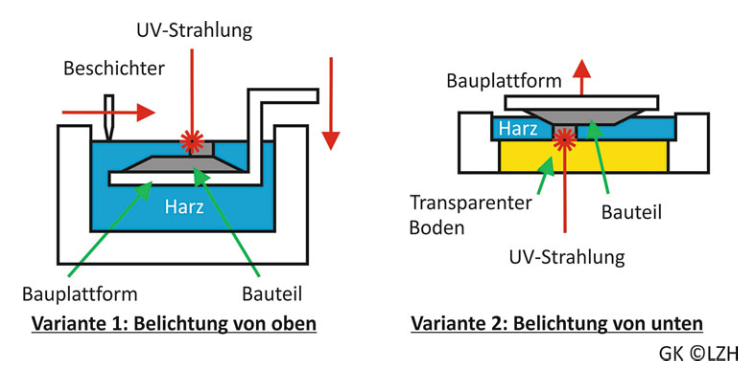
\includegraphics[width=.5\textwidth]{images/SdT/verfahren/UVStereolith_lach16}}
 		\picskip{0}
 		\vspace*{3em}
		
		F�r jede Schicht kann eine Photomaske erzeugt werden. Der fl�ssige Grundstoff wird durch die Maske hindurch von einer \ac{UV}- Quelle angestrahlt. Dadurch h�rtet eine Schicht des Grundmaterials entsprechend der Photomaske aus. Die erste Schicht wird auf eine Bodenplatte gedruckt. Diese wird nach Abschlie�en jeder Schicht weiter in die Fl�ssigkeit abgesenkt. Dadurch wird die n�chste Schicht auf die darunterliegende gedruckt.
		
		
		Alternativ zur Photomaske mit gleichm��iger Quelle kann auch ein \ac{UV}- Laser verwendet werden, der �ber Spiegel an die auszuh�rtenden Rasterpunkte gelenkt wird.
		
		Das erzeugte Objekt wird im Druckverfahren nicht vollst�ndig ausgeh�rtet. Daher muss es im Anschluss mit \ac{UV}- Licht nachbehandelt werden.
		\cite[S.3]{gebhardt2004grundlagen}
	
	\subsection{Sintern}
		 Sintern beschreibt den Prozess des Verdichtens pulverf�rmiger Ausgangsstoffe zu einem festen Material. Hierzu kann das Material �ber den Schmelzpunkt erhitzt werden oder durch hohe Dr�cke dazu verleitet werden, dass sich die Oberfl�chen der einzelnen Pulverk�rner verbinden.
		 F�r den \ac{3D}- Druck relevant sind Verfahren, die ein selektives Verbinden der K�rner erm�glichen.
		 \cite[Bd.20, S.7037]{meyers2006}
		 
		 %	\subsubsection{Elektronenstrahlschmelzen}
		 Ein Verfahren, das dies erm�glicht, ist das Elektronenstrahlschmelzen. Hierbei wird schichtweise das Pulver des Ausgangsmaterials selektiv mit einem Elektronenstrahl geschmolzen. Nach Fertigstellung einer Schicht wird eine weitere Schicht Pulver aufgetragen, die erneut selektiv geschmolzen werden kann. Dadurch k�nnen \ac{3D} Objekte erzeugt werden. Momentan sind Objekte aus mehreren Titanlegierungen mit diesem Verfahren m�glich. Zudem wird an der Eignung von Stahl, verschiedenen Metallen und deren Legierungen geforscht.
		 \cite{IFAMElektronenstrahl}
		 
 		\piccaption{Funktionsweise des Elektronenstrahlschmelzens \cite{lachmayer3d}\label{fig:sdt:estrahlschmelzen}}
 		\parpic{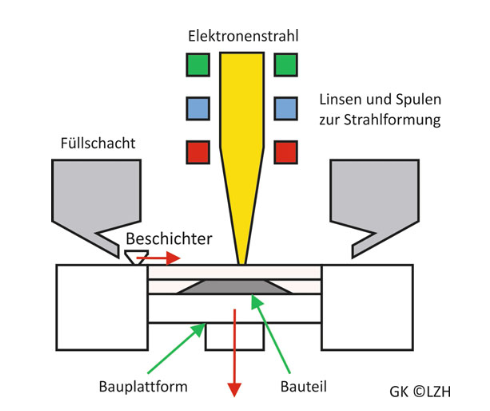
\includegraphics[width=.6\textwidth]{images/SdT/verfahren/EStrahl_lach16}}
 		\picskip{0}
 		\vspace*{3em}
 		
		 
		 %\subsubsection{Lasersintern}
		 Alternativ zum Elektronenstrahl kann auch ein Laser zum Verschwei�en des Pulvers eingesetzt werden. Mit diesem Verfahren k�nnen auch Kunststoffe verarbeitet werden. 	
		\cite{lasersintern}
		
		\piccaption{Prinzip des selektiven Lasersinterns \cite{lachmayer3d}\label{fig:sdt:laserschmelzen}}
		\parpic{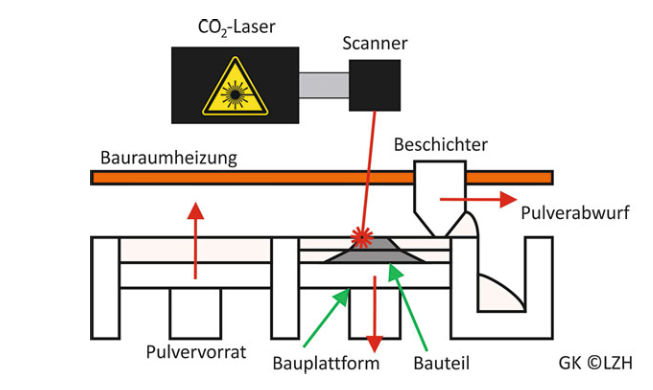
\includegraphics[width=.5\textwidth]{images/SdT/verfahren/selLaserSintern_lach16}}
 		\picskip{0}
 		\vspace*{3em}
		
	\subsection{Binder-Verfahren}
		Im Binderverfahren wird ein Bindemittel in ein pulverf�rmiges Ausgangsmaterial eingespritzt. Durch selektives Einbringen des Binders k�nnen die gew�nschten Strukturen erzeugt werden.
		\cite[S.11]{gebhardt2004grundlagen}
		
	\subsection{Schicht-Laminat-Verfahren}
	\label{drucktechniken:schichtLaminatVerfahren}
		In jeder Schicht wird ein Metallblech mit einem Laser in Form geschnitten. Die fertigen Schichten werden verpresst, verklebt oder versintert. Dadurch entsteht ein geschichtetes Objekt, dessen Eigenschaften sich in Faserrichtung von denen gegen Faserrichtung unterscheiden.\cite[S.33]{hagl2014_3DKompendium}
		
		\piccaption{Funktionsweise des Schicht-Laminat-Verfahrens \cite{gebhardt2004grundlagen}\label{fig:sdt:schichtLaminat}}
		\parpic{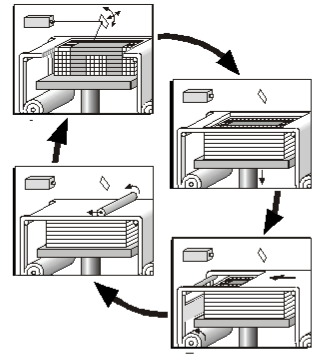
\includegraphics[width=.5\textwidth]{images/SdT/verfahren/schichtLam_gebGr}}
 		\picskip{0}
 		\vspace*{3em}
		
		
		

\section{Materialien}
	Die verschiedenen Druckverfahren erfordern unterschiedliche Grundstoffe f�r das Drucken. Dieser Abschnitt stellt verschiedene Materialien vor.
	
	\subsection{Metalle und deren Legierungen}
		Pulver verschiedener Metalle und Legierungen lassen sich sintern. Bleche k�nnen im Schicht-Lamitat-Verfahren \ref{drucktechniken:schichtLaminatVerfahren} zu einem festen Objekt geformt werden. Im Allgemeinen lassen sich aus Metall per 3D- Druck mechanisch und thermisch belastbare Prototypen erstellen.
	\subsection{Monomere}
		Im Stereolithographie-Verfahren \ref{drucktechniken:stereolithographie} werden Monomere selektiv polymerisiert. Monomere sind Molek�le, die mit gleichartigen Molek�len zu gr��eren Molek�len verschmelzen k�nnen. Durch Polymerisation entsteht ein fester K�rper aus langkettigen Molek�len. 
		\cite{Abts2014Polymere}
		
	\subsection{Thermoplaste}
		Bereits polymerisierte Kunststoffe unterscheiden sich in der Reaktion auf hohe Temperaturen. Eine dieser Gruppen von Polymeren sind die Termoplaste. Diese Kunststoffe verfl�ssigen sich bei Temperatureinwirkung und erstarren beim anschlie�enden Ausk�hlen in einer neuen Form. Wenn die Temperatur zu hoch ist, verschmoren Thermoplaste. Daher muss beim Drucken eine Temperatur gefunden werden, die das Material in eine verwendbare Liquidit�t versetzt, allerdings das Material nicht besch�digt. Bekannte Thermoplaste sind \ac{PLA} und \ac{ABS}. Ebenfalls l�sst sich Schokolade drucken. Beim Drucken mit \ac{ABS} entstehen giftige D�mpfe. Die Menge an ausgeschiedenem Gas ist bei korrekter Druckertemperatur-Einstellung unbedenklich, allerdings sollte der Druckraum trotzdem gut ventiliert werden.
		
		Im Gegensatz zu den Thermoplasten verfl�ssigen sich Duroplaste nicht; sie verschmoren direkt, wenn die Temperatur zu hoch wird. Dadurch eignen sie sich nicht f�r das Extrusionsverfahren.  

\section{Stabilit�tsanalyse}
In diesem Kapitel wird betrachtet, wie stabil die Objekte sind, die mit den vorgestellten Verfahren hergestellt werden. 

\subsection{Extrusionsverfahren} %TODO
%gebh: + mech+therm bel h�her als stereol, -raue oberfl, geringere details

\subsection{Stereolithographie}
Objekte, die mit Stereolithografie hergestellt werden, sind mechanisch und thermisch weniger belastbar als Objekte, die beispielsweise mit Lasersintern oder im Extrusionsverfahren hergestellt wurden. \cite{gebhardt2004grundlagen}\\
Zudem ist unklar, ob diese Objekte stabil genug f�r einen Dauereinsatz sind. \cite{hagl2014_3DKompendiumTechnologien}
% fl�ssig: ungenau
% nachbehandlung
% langfristige Stabilit�t "Sorgenpunkt"
% + gro�e objekte, hohe pr�zision, oberfl�chenveredlung 

%Gebhardt: -mech + therm belastbarkeit schlcehter als lasersintern/extrusion

\subsection{Elektronenstrahlschmelzen}  %TODO

\subsection{Lasersintering}
Dieses Verfahren kann sowohl Metall als auch Kunststoff verarbeiten. Die dabei produzierten Teile k�nnen �hnliche Eigenschaften wie herk�mmlich produzierte Teile aufweisen.    \\
Allerdings sind gesinterte Teile por�s, was bei manchen Anwendungsf�llen erw�nscht sein kann. Die Porosit�t kann abgeschw�cht werden, indem das Pulver mit anderen Materialien versetzt wird. \cite{hagl2014_3DKompendiumTechnologien}


% \subsection{Binder-Verfahren}  %TODO
\subsection{Schicht-Laminat-Verfahren}
Da bei diesem Verfahren die Objekte aus verschiedenen Schichten aufgebaut sind, die miteinander verpresst oder verklebt wurden, weisen diese Objekte richtungsabh�ngig verschiedene Eigenschaften auf.
\cite{gebhardt2004grundlagen}
%gebh: -richtungsabh. eigenschaften, geringere genauigkeit


\section{\acf{CAD}}
	
	%TODO Einleitung CAD
	Der 3D-Druck basiert zum gro�en Teil auf dem computergest�tzten Design von Objekten. \ac{CAD}-Tools helfen beim Entwerfen. Anschlie�end werden die Objektdateien mithilfe von Slicern in 	maschinenlesbaren Code umgewandelt. Die Unterkapitel stellen die verwendeten Programme vor.
		
	\subsection{CAD-Programme}
		
		F�r das Design von 3D-Dateien gibt es vielerlei Programme. Auf kostenloser Basis wurden in dieser Arbeit Solid Edge und blender verwendet. 
		
		\subsubsection{Solid Edge}
			

			\piccaption{Screenshot des Programms blender\label{fig:sdt:solidEdge}}
			\parpic{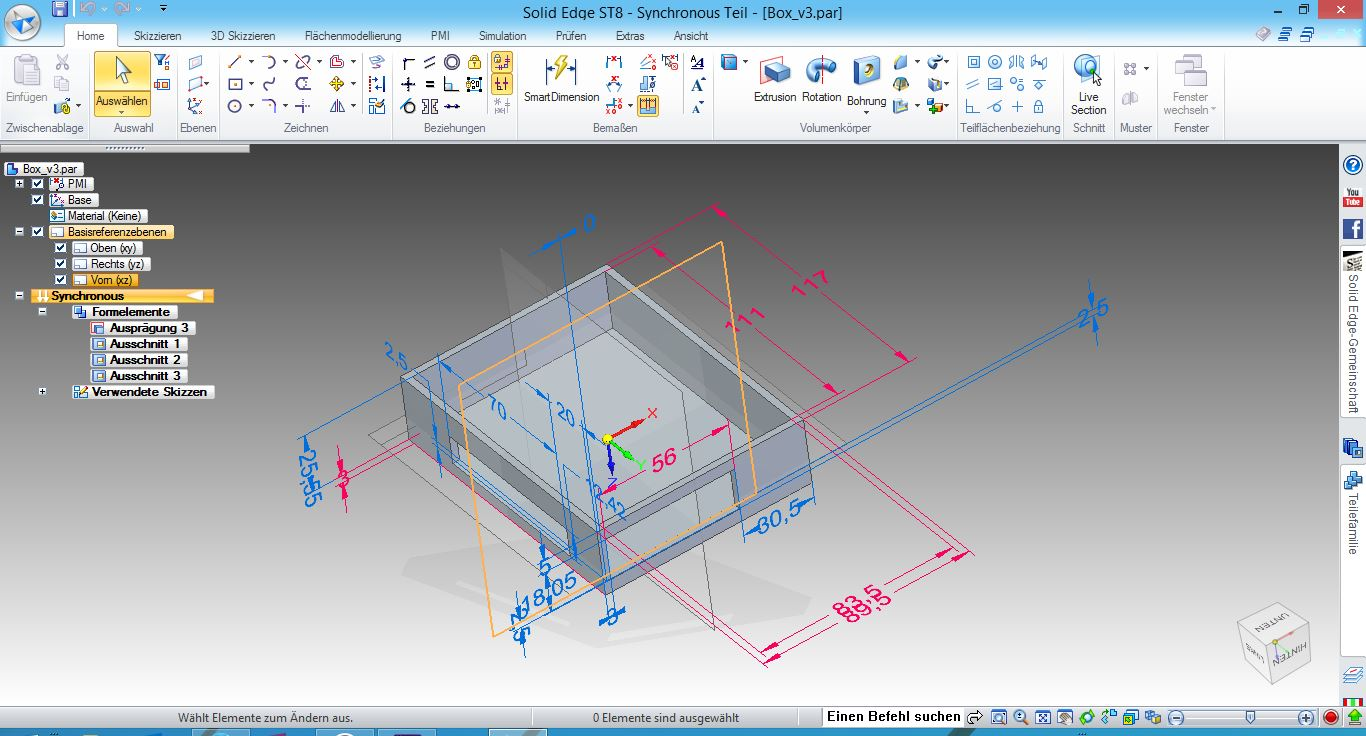
\includegraphics[width=.5\textwidth]{images/SdT/solidEdge}}
			
			Solid Edge von Siemens eignet sich f�r das Entwerfen von technischen Objekten. Hierbei bietet das Programm eine Vielzahl von Funktionen f�r die Erstellung von 2D- und 3D-Formen. F�r einfache Objekte kann eine 2D-Grundform gezeichnet und anschlie�end zu einem 3D-Objekt extrahiert werden. Zus�tzliche Funktionen von Solid Edge unterst�tzen bei der Stabilit�tsanalyse der entwickelten Objekte.
			
			Die Entwicklung der Objekte kann entweder auf sequenzieller Basis oder auf paralleler Basis geschehen. Die sequenzielle Entwicklung erfordert ein hohes Ma� an Programmkenntnis, da die einzelnen Schritte der Objekterstellung nur in einem definierten Ablauf stattfinden kann. Der parallele Entwicklungsstack erleichtert die nachtr�gliche Ver�nderung von Arbeitsschritten wie zum Beispiel die Ma�e, die w�hrend einer Extraktion angegeben wurden. Zus�tzlich k�nnen bei paralleler Entwicklung die Renderzeiten bei Ma��nderungen deutlich reduziert werden. Das zahlt sich bei umfangreichen Objekten aus.
			
			F�r die Arbeit wurde die akademische Lizenz verwendet. Objekte, die mit dieser Lizenz erstellt wurden, k�nnen nicht mit einer anderen Lizenz ge�ffnet werden.
			
			
		\subsubsection{blender}
			
			\piccaption{Screenshot des Programms blender\label{fig:sdt:blender}}
			\parpic{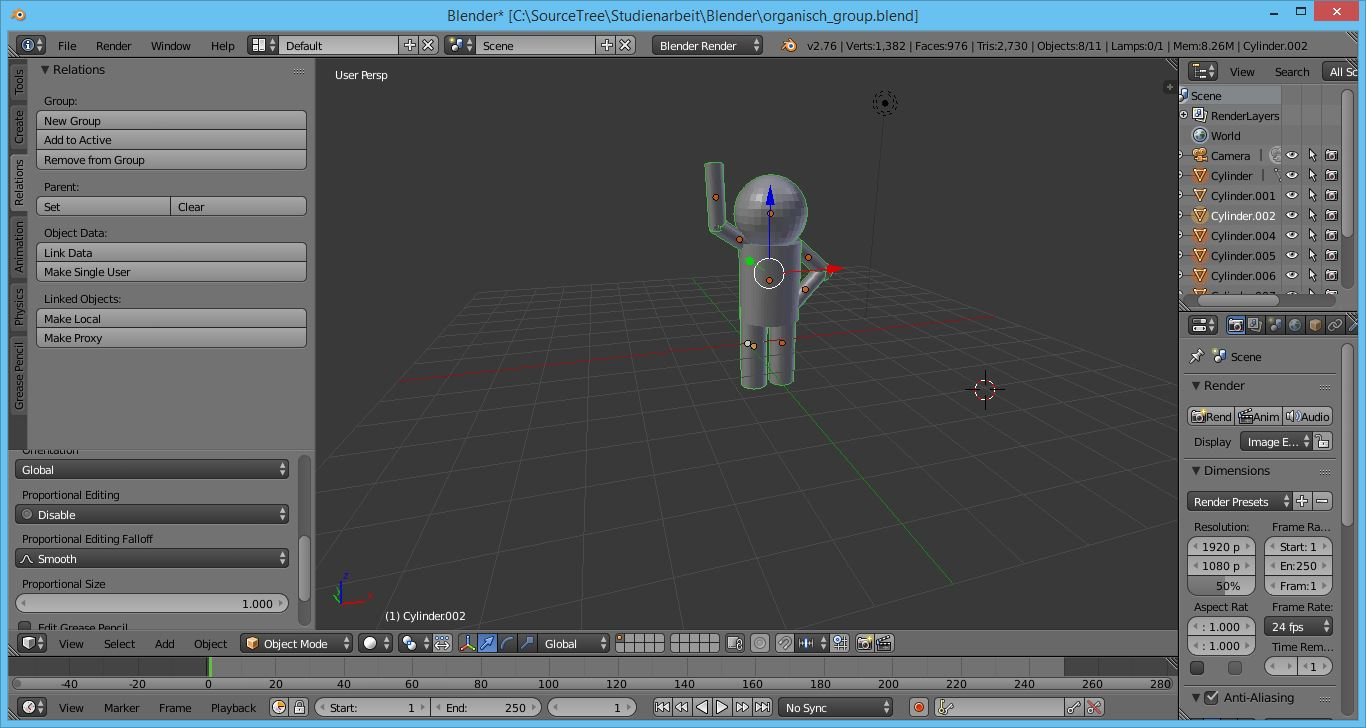
\includegraphics[width=.5\textwidth]{images/SdT/blender}}
			
			Blender ist ein Open Source Programm, das eine Vielzahl von Computergrafik-Anwendungen bietet. Diese reichen von der Erstellung von Objekten bis hin zum Filmschnitt.
			
			Die CAD-Funktionen zielen vor allem auf die Animation einzelner Objekte ab. Zum Beispiel kann die Beweglichkeit der Finger mit Regeln definiert werden. Das Objekt-Design unterliegt der Manipulation von Basis-Objekten, die dann anschlie�end zu einem Objekt vereinigt werden.
			
		
		\subsection{Slicing}
			
			Das Slicing ist der Prozess zur Umwandlung eines 3D-Objekts in f�r den Drucker eindeutige Befehle. Da jeder Drucker unterschiedliche Randbedingungen bietet, empfielt der jeweilige Hersteller ein f�r den Drucker geeignetes Programm zum Slicen.
			
			Der 3D-Drucker Ultimaker 2 erh�lt seine Dateien vom Ultimaker eigenen Programm Cura. Alternativ kann das Programm Repertierhost verwendet werden.
			
		\subsubsection{Cura}

			
			\piccaption{Screenshot des Programms blender\label{fig:sdt:cura}}
			\parpic{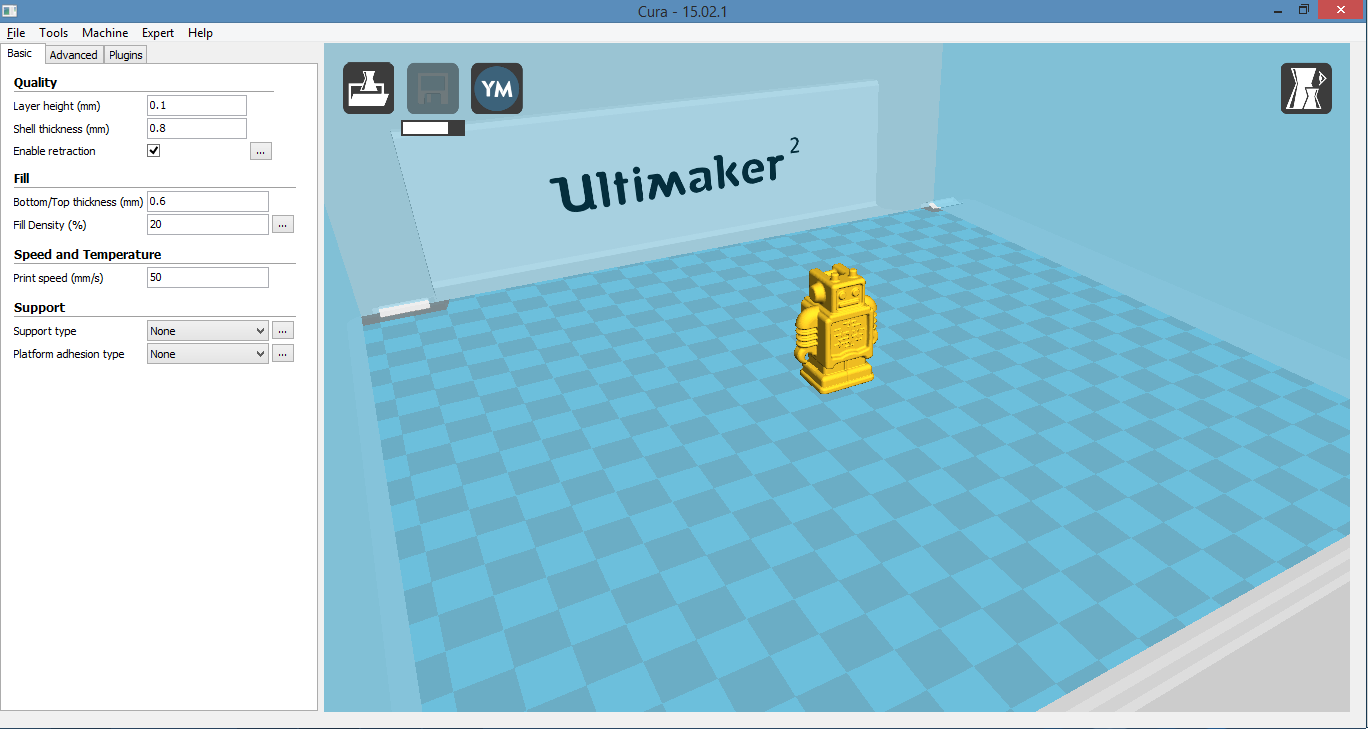
\includegraphics[width=.5\textwidth]{images/SdT/cura}}
			
			Mit Cura kann man aus Objektdateien im \ac{STL}-Format G-code f�r den Ultimaker erstellen. Das Programm erlaubt die Variation zahlreicher Parameter, die den Druck beeinflussen. Die verwendete Programmversion beeinflusst die Ergebnisse des Slicens deutlich. Viele Druckoptionen sind erst mit neueren Versionen m�glich. Eine wichtige fehlende Funktion von Cura ist eine Einstellm�glichkeit der Drucktemperatur. Der Befehl ist im G-code vorgesehen, allerdings nicht beeinflussbar.
			
		\subsubsection{Repetierhost}
			
			
			\piccaption{Screenshot des Programms blender\label{fig:sdt:repetierhost}}
			\parpic{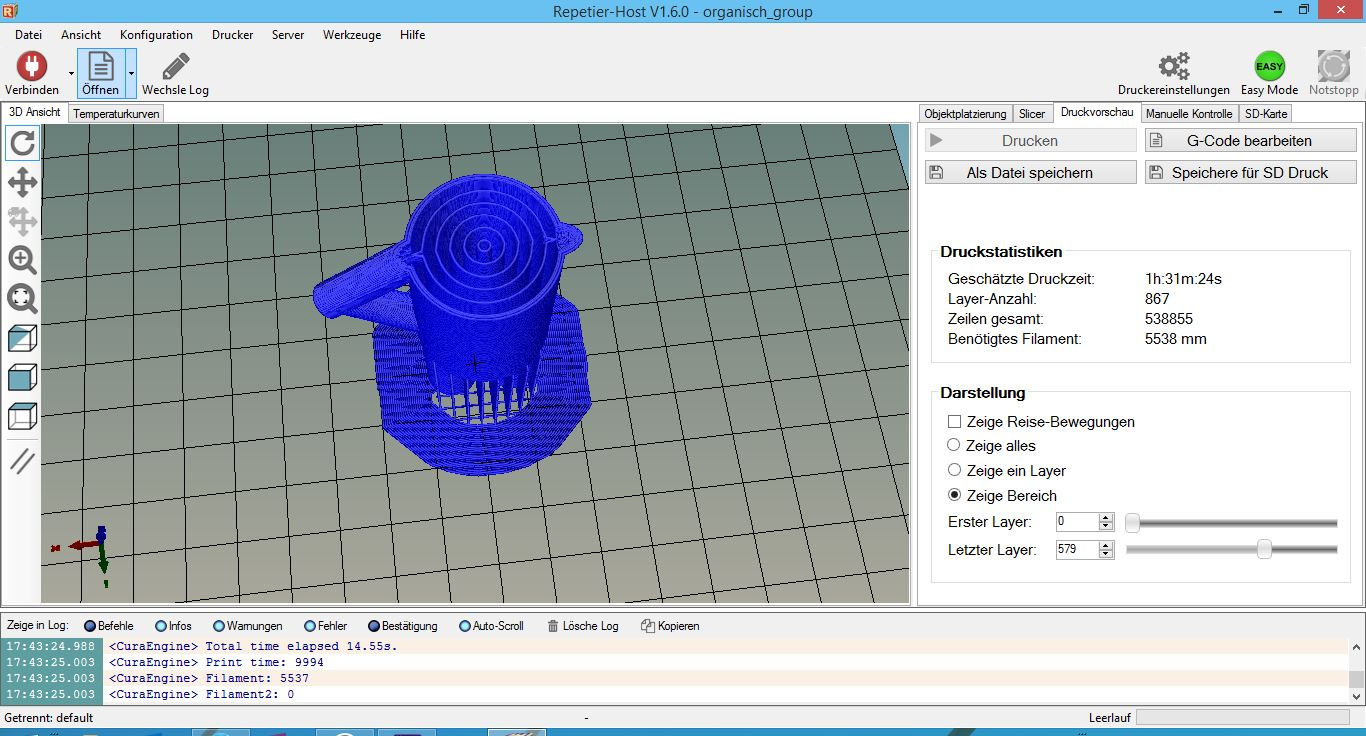
\includegraphics[width=.5\textwidth]{images/SdT/repetierhost}}
			
			Repetierhost ist ein alternatives Programm zur Fernsteuerung von 3D-Druckern. Es visualisiert Druckdateien im \ac{STL}- und im G-code-Format. Zudem enth�lt es einen Slicer, mit dem man selbigen erzeugen kann. 
			
			Cura liefert mitunter fehlerhaften G-code, in dem L�cher klaffen oder Schichten fehlen. Mithilfe des Repetierhosts k�nnen diese Fehler entdeckt werden.
			
	\subsection{Dateiformate}
		
		F�r die Darstellung von 3D-Objekten k�nnen verschiedene Datentypen verwendet werden. Essenziell f�r den 3D-Druck mit dem Ultimaker sind die Dateitypen \ac{STL} und der G-code.
		
		\subsubsection{\acf{STL}}
			
			Eine \ac{STL}-Datei ist eine Oberfl�chendefinition f�r ein 3D-Objekt. Hierf�r werden die dreieckigen orientierten Facetten �ber ihre Eckpunkte in einem kartesischen Koordinatensystem abgespeichert. Die Dimensionierung(z.B. Zentimeter oder Inch) wird nicht mit abgespeichert und muss vom lesenden Programm eingestellt werden.
			
			Da das STL-Format eine einfache Objektbeschreibung ist, kann es als universelle Schnittstelle zwischen \ac{CAD}-Designprogrammen und Slicern verwendet werden. Allerdings gehen Zusatzinformationen wie unterschiedlich eingestellte Drucktemperaturen oder Druckfarben verloren. Daher eignet sich das Format nur zur �bergabe von  einfachen Formeigenschaften.			
			
		\subsubsection{G-code}
			
			Aus der Welt der Fr�sen kommend ist der G-code eine Sprache, mit der Maschinen Positionierungs- und Arbeitsanweisungen erhalten k�nnen. 
			
			Derivate dieser Sprache wurden um die Funktionen zur Steuerung eines 3D-Druckers erweitert. Mithilfe der neuen Befehle k�nnen zum Beispiel die Drucktemperatur oder die L�fter angesteuert werden.
			
			
	
\section{ZTemperaturtestdrcuk}
	
	\begin{figure}[h!]
		
		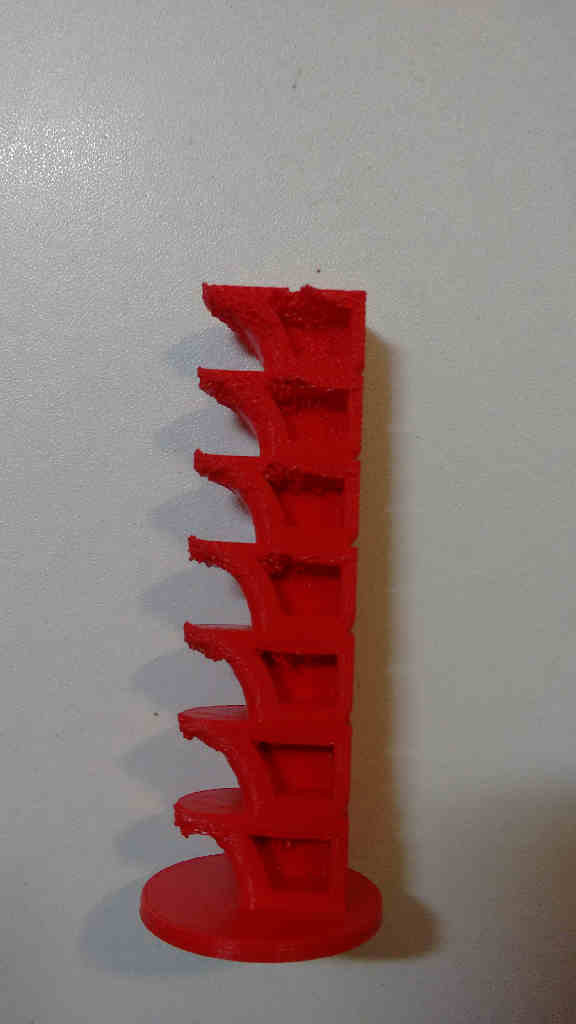
\includegraphics[height=20em]{images/techGr/Temperaturtest}
		\hspace*{1em}
		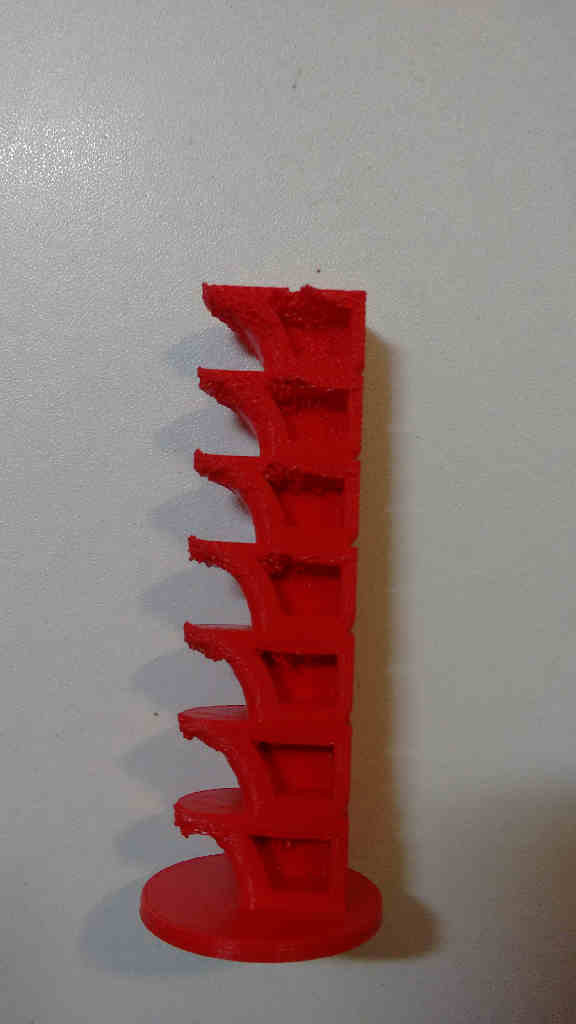
\includegraphics[height=20em]{images/techGr/Temperaturtest}
		\caption[Temperaturtest]{Temperaturtestdruck}
		\label{grafik:techGr:Temperaturtest}
	\end{figure}
	
	
	bfuesg \\
	busp
	\piccaption[Temperaturtest]{asdf \label{grafik:techGr:Temperaturtest1}}
	\parpic{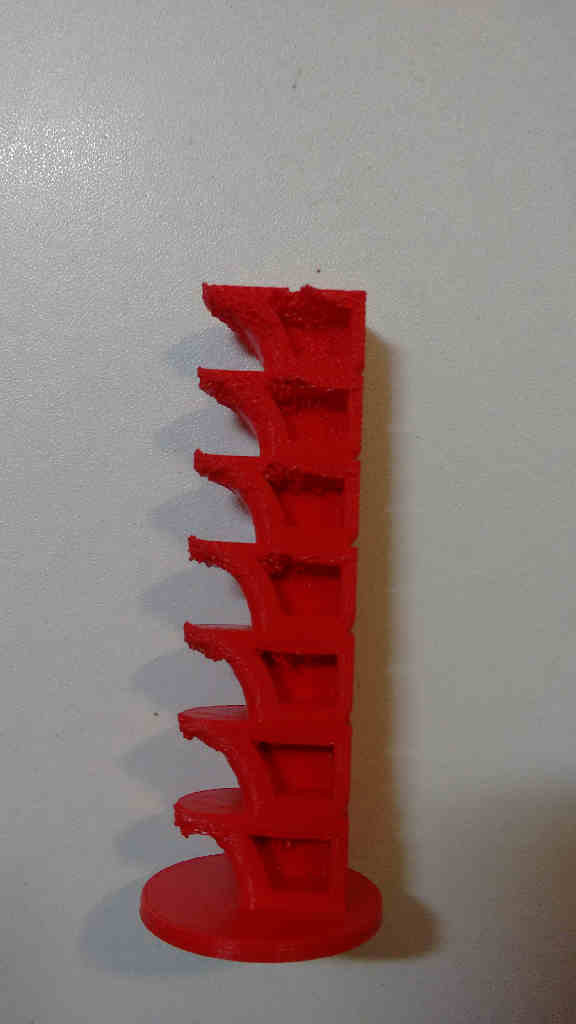
\includegraphics[height=20em]{images/techGr/Temperaturtest}}
	%\picskip{0} 
	buepsgb 
	\vspace*{1em}
	bsueb\\
	\picskip{0}
	
	
	
\section{Der \ac{3D}-Drucker Ultimaker 2}
	\label{chapter:techGr:ultimaker2}
	.
	% Bilder Ultimaker
	% Quelle Ultimaker Website
	

	
	...
	